\documentclass[12pt, twoside]{book}
%\documentclass[12pt, oneside]{book}  % jednostranna tlac

%spravne nastavenie okrajov
\usepackage[a4paper,top=2.5cm,bottom=2.5cm,left=3.5cm,right=2cm]{geometry}
%zapnutie fontov pre UTF8 kodovanie
\usepackage[utf8]{inputenc}
\usepackage[T1]{fontenc}

%zapnutie slovenskeho delenia slov
%a automatickych nadpisov ako Obsah, Obrázok a pod. v slovencine
%\usepackage[slovak]{babel} % vypnite pre prace v anglictine!

%nastavenie riadkovania podla smernice
\linespread{1.25} % hodnota 1.25 by mala zodpovedat 1.5 riadkovaniu

% balicek na vkladanie zdrojoveho kodu
\usepackage{listings}
% ukazky kodu su cislovane ako Listing 1,2,...
% tu je Listing zmenene na Algoritmus 1,2,...
\renewcommand{\lstlistingname}{Algorithm}
% nastavenia balicka listings
% mozete pridat aj language=...
% na nastavenie najcastejsie pouzivaneho prog. jazyka
% takisto sa da zapnut cislovanie riadkov
\lstset{frame=lines}

% balicek na vkladanie obrazkov
\usepackage{graphicx}
% balicek na vkladanie celych pdf dokumentov, tu zadanie
\usepackage{pdfpages}
% balicek na spravne formatovanie URL
\usepackage{url}
% balicek na hyperlinky v ramci dokumentu
% zrusime farebne ramiky okolo liniek aby pdf
% vyzeralo rovnako ako tlacena verzia
\usepackage[hidelinks,breaklinks]{hyperref}


% -------------------
% --- Definicia zakladnych pojmov
% --- Vyplnte podla vasho zadania, rok ma byt rok odovzdania
% -------------------
\def\mfrok{2024}
\def\mfnazov{Automatic Human Anthropometric Body Measurements Estimation}
\def\mftyp{Bachelor Thesis}
\def\mfautor{Michal Baránek}
\def\mfskolitel{Mgr. Dana Škorvánková}

%ak mate konzultanta, odkomentujte aj jeho meno na titulnom liste
\def\mfkonzultant{tit. Meno Priezvisko, tit. }  

\def\mfmiesto{Bratislava, \mfrok}

% študenti BIN a DAV odkomentujú príslušnú dvojicu riadkov
\def\mfodbor{Computer Science}
\def\program{Computer Science }

% Ak je školiteľ z FMFI, uvádzate katedru školiteľa, zrejme by mala byť aj na zadaní z AIS2
% Ak máte externého školiteľa, uvádzajte Katedru informatiky 
\def\mfpracovisko{ Department of Computer Science }

\begin{document}     
\frontmatter
\pagestyle{empty}

% -------------------
% --- Obalka ------
% -------------------

\begin{center}
  \sc\large
  Comenius University in Bratislava\\
  Faculty of Mathematics, Physics and Informatics

\vfill

{\LARGE\mfnazov}\\
\mftyp
\end{center}

\vfill

{\sc\large 
\noindent \mfrok\\
\mfautor
}

\cleardoublepage
% --- koniec obalky ----

% -------------------
% --- Titulný list
% -------------------

\noindent

\begin{center}
\sc  
\large
  Comenius University in Bratislava\\
  Faculty of Mathematics, Physics and Informatics

\vfill

{\LARGE\mfnazov}\\
\mftyp
\end{center}

\vfill

\noindent
\begin{tabular}{ll}
Study Programme: & \program \\
Field of Study: & \mfodbor \\
Department: & \mfpracovisko \\
Supervisor: & \mfskolitel \\
% Consultant: & \mfkonzultant \\
\end{tabular}

\vfill


\noindent \mfmiesto\\
\mfautor

\cleardoublepage
% --- Koniec titulnej strany


% -------------------
% --- Zadanie z AIS
% -------------------
% v tlačenej verzii s podpismi zainteresovaných osôb.
% v elektronickej verzii sa zverejňuje zadanie bez podpisov
% v pracach v anglictine anglicke aj slovenske zadanie

\newpage
\setcounter{page}{2}
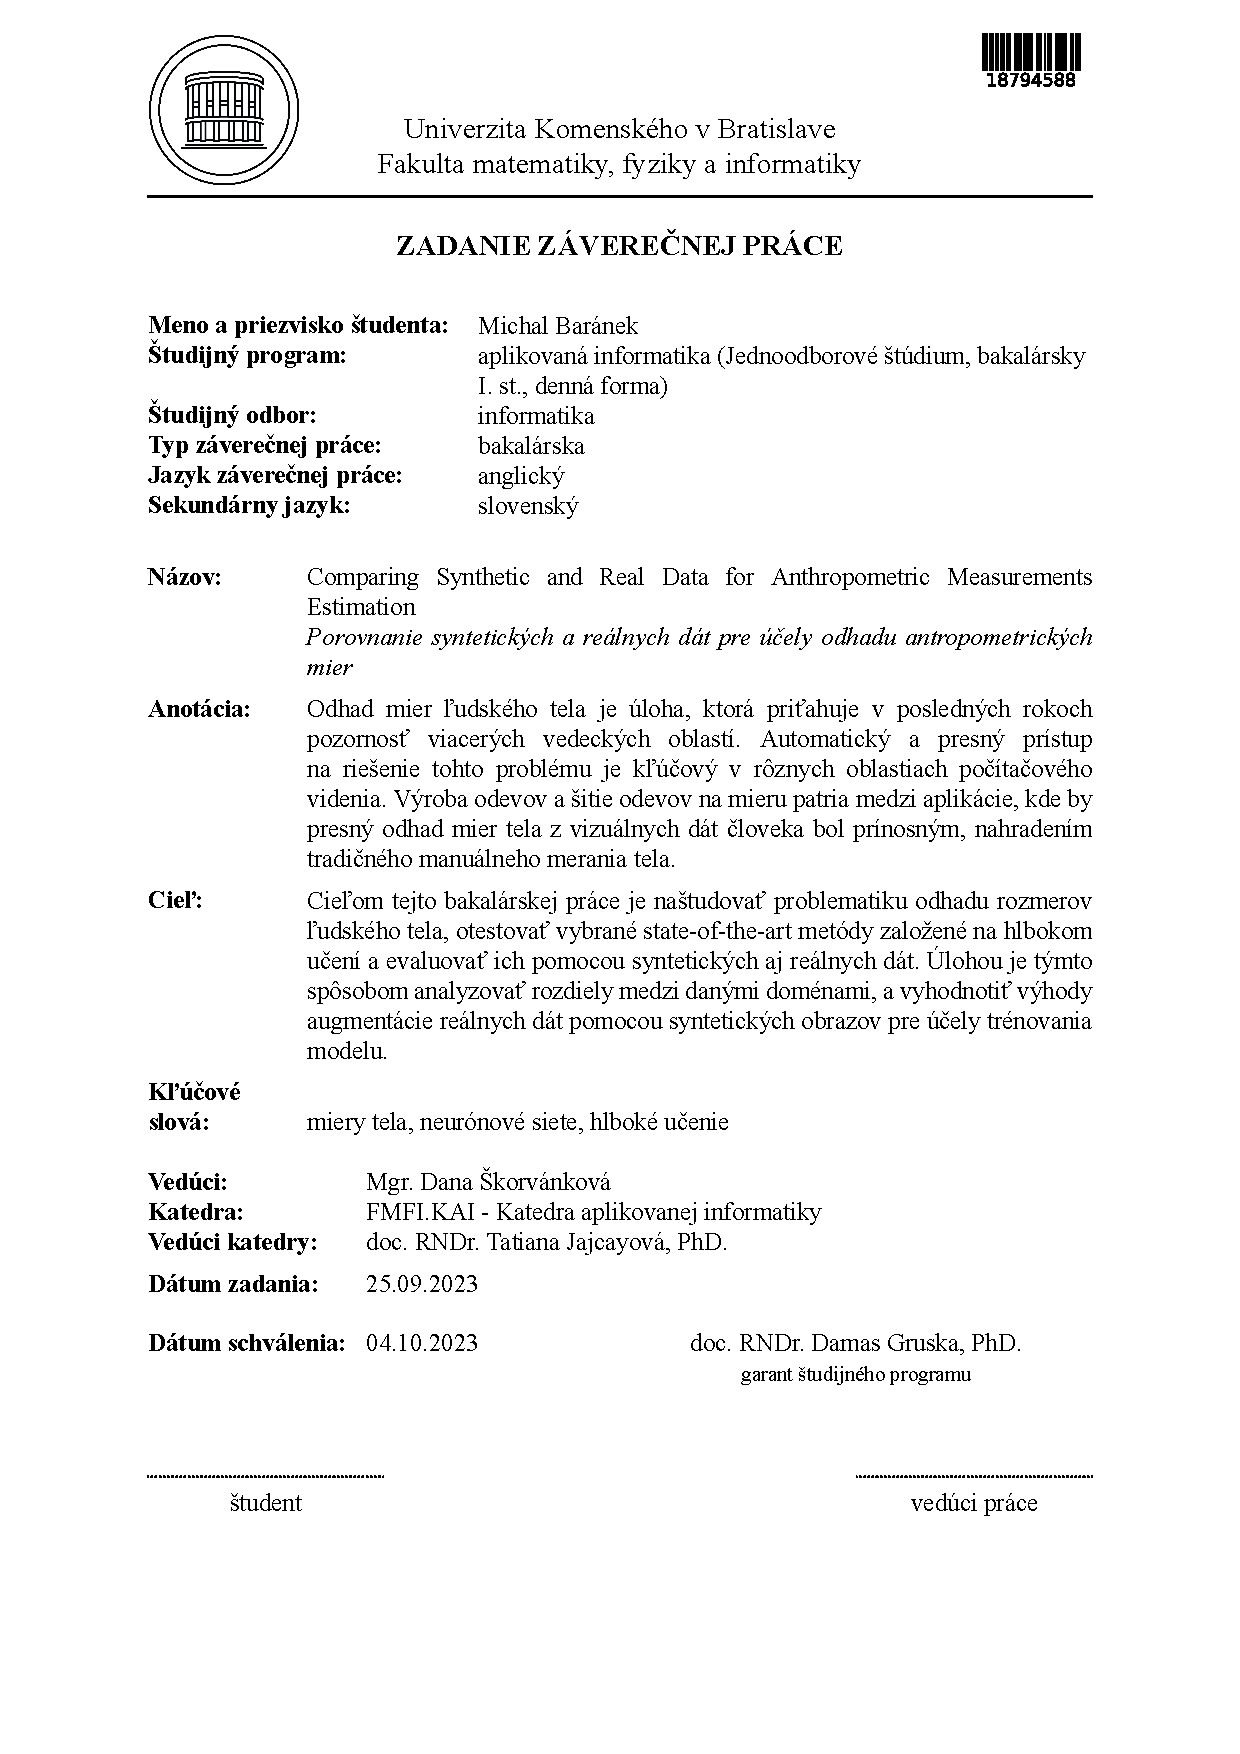
\includepdf{images/zadanie.pdf}

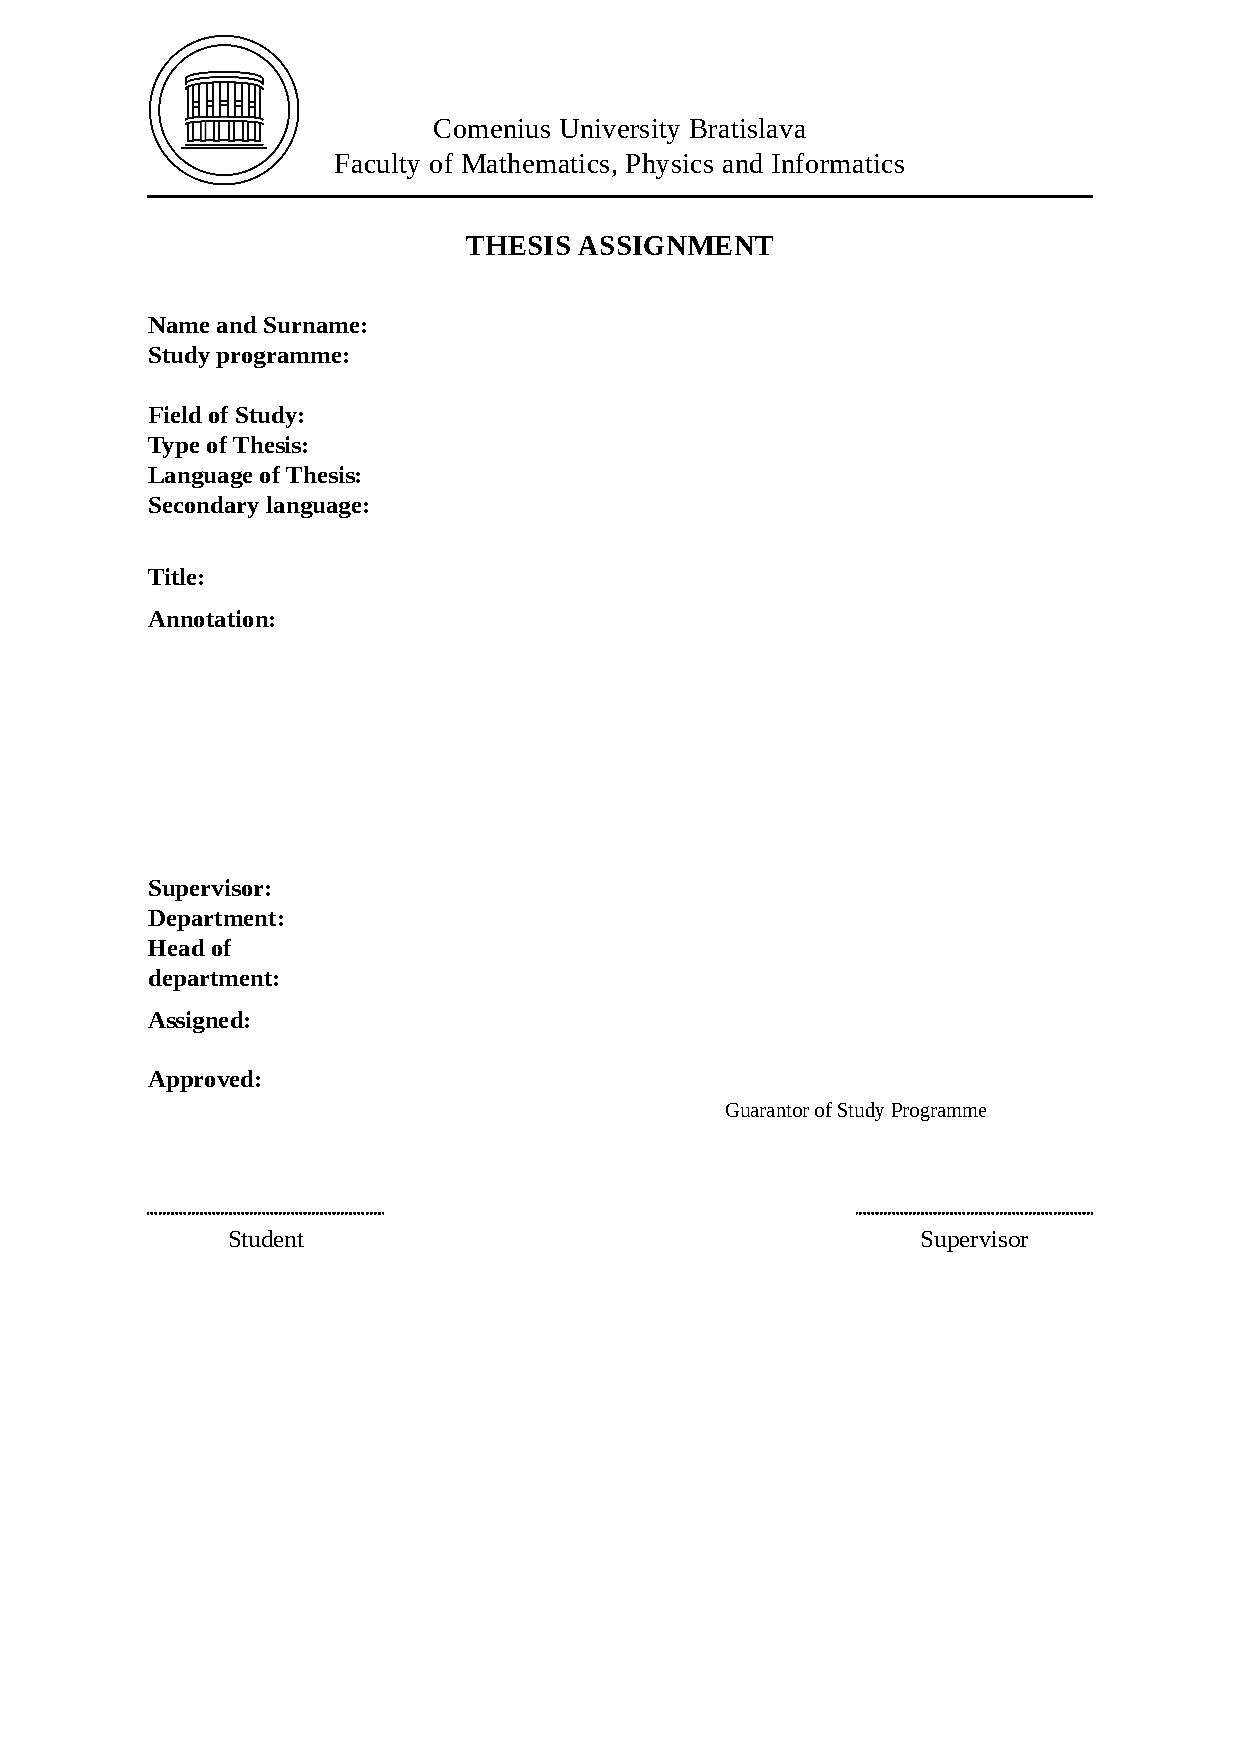
\includepdf{images/zadanie-en.pdf}

% --- Koniec zadania


% -------------------
%   Poďakovanie - nepovinné
% -------------------
\newpage
\pagestyle{plain}
~

\vfill
{\bf Acknowledgments:} Tu môžete poďakovať školiteľovi, prípadne
ďalším osobám, ktoré vám s prácou nejako pomohli, poradili,
poskytli dáta a podobne.

% --- Koniec poďakovania

% -------------------
%   Abstrakt - Slovensky
% -------------------
\newpage 
\section*{Abstrakt}


Slovenský abstrakt v rozsahu 100-500 slov, jeden odstavec. Abstrakt
stručne sumarizuje výsledky práce. Mal by byť pochopiteľný pre bežného
informatika. Nemal by teda využívať skratky, termíny alebo označenie
zavedené v práci, okrem tých, ktoré sú všeobecne známe.

\paragraph*{Kľúčové slová:} jedno, druhé, tretie (prípadne štvrté, piate)
% --- Koniec Abstrakt - Slovensky


% -------------------
% --- Abstrakt - Anglicky 
% -------------------
\newpage 
\section*{Abstract}

Abstract in the English language (translation of the abstract in the
Slovak language).


\paragraph*{Keywords:} 

% --- Koniec Abstrakt - Anglicky

% -------------------
% --- Predhovor - v informatike sa zvacsa nepouziva
% -------------------
%\newpage 
%
%
%\chapter*{Preface} %
%
%Predhovor je všeobecná informácia o práci, obsahuje hlavnú charakteristiku práce 
%a okolnosti jej vzniku. Autor zdôvodní výber témy, stručne informuje o cieľoch 
%a význame práce, spomenie domáci a zahraničný kontext, komu je práca určená, 
%použité metódy, stav poznania; autor stručne charakterizuje svoj prístup a svoje
%hľadisko. 
%
% --- Koniec Predhovor


% -------------------
% --- Obsah
% -------------------

\newpage 

\tableofcontents

% ---  Koniec Obsahu

% -------------------
% --- Zoznamy tabuliek, obrázkov - nepovinne
% -------------------

\newpage 

\listoffigures
\listoftables

% ---  Koniec Zoznamov

\mainmatter
\pagestyle{headings}

%\input uvod.tex 

%\input kapitola.tex

%\input latex.tex

\addcontentsline{toc}{chapter}{Introduction}
\chapter*{Introduction}
Nowadays our physical bodies are not enough for us anymore. Thanks to modern technologies every day we come closer to living a new type of life. Virtual one. The beginnings were quite humble with us sharing our thoughts via text and shortly after empowering our life stories with images. Thanks to these innovations we were able to create a new type of business - online shops. Their popularity rose over the years and are now rivals to traditional ways of shopping. These new online stores however have a significant disadvantage in comparison. You cannot try the clothes on and see whether it will fit. Luckily we have already created clothing sizing system to help us choose the correct size. However to use this system one would need exact body measurements to look up correct size in the table. \\ \\
Online shops however were not the only blooming business in recent years. A new prospect has appeared only just recently and it caught attention of big companies straight away. The virtual world where we could meet our friends living anywhere in the world without having to leave our home. In this world everyone would have their own avatar that would represent them. Some virtual worlds would let you become whoever or even whatever you could possibly think of while some others decided to stick with realism. Realism sounds great, but this approach requires realistic data to be able to look convincing. To create a clone of human body in the virtual world we amongst many variables would need exact body measurements to provide a believable result.\\ \\
These are just two examples that require users to obtain their body measurements. While the act of measuring does not seem very problematic the measurements are prone to human error. There are no rules when it comes to measuring body parts. Usually, subjects are only guided via text or image showing them how to measure. This will never satisfy the accuracy that is required.\\ \\
Thanks to progress in neural networks a new way of obtaining body measurements has emerged. With requiring only picture of body from front we can train a neural network to predict measurements of human body. This has already been proven plausible, but the accuracy lacked in some measurements. The goal of this work is to compare different .... (To make data better). The methods will vary to see how impactful they are regarding the final result.\\\\
For training we will use a synthetic dataset which will allow us to have much larger number of samples for training. For metrics we will use performance on dataset with real samples provided by BodyM dataset.\\\\
The first chapter will provide overview of the problematic, will look into traditional measuring methods, delve into obstacles this approach faces and then explain some of the mechanical works of this thesis. Second chapter will look into already existing work that is relevant to topic. In the third chapter we will define datasets. Contents of fourth chapter will focus on proposed solution and implementation. Results of our research will be located in fifth chapter while the sixth chapter will provide conclusion.


%\input zaver.tex

% -------------------
% --- Bibliografia
% -------------------


\newpage	

\backmatter

\thispagestyle{empty}
\clearpage

\bibliographystyle{plain}
\bibliography{literatura} 

%Prípadne môžete napísať literatúru priamo tu
%\begin{thebibliography}{5}
 
%\bibitem{br1} MOLINA H. G. - ULLMAN J. D. - WIDOM J., 2002, Database Systems, Upper Saddle River : Prentice-Hall, 2002, 1119 s., Pearson International edition, 0-13-098043-9

%\bibitem{br2} MOLINA H. G. - ULLMAN J. D. - WIDOM J., 2000 , Databasse System implementation, New Jersey : Prentice-Hall, 2000, 653s., ???

%\bibitem{br3} ULLMAN J. D. - WIDOM J., 1997, A First Course in Database Systems, New Jersey : Prentice-Hall, 1997, 470s., 

%\bibitem{br4} PREFUSE, 2007, The Prefuse visualization toolkit,  [online] Dostupné na internete: <http://prefuse.org/>

%\bibitem{br5} PREFUSE Forum, Sourceforge - Prefuse Forum,  [online] Dostupné na internete: <http://sourceforge.net/projects/prefuse/>

%\end{thebibliography}

%---koniec Referencii

% -------------------
%--- Prilohy---
% -------------------

%Nepovinná časť prílohy obsahuje materiály, ktoré neboli zaradené priamo  do textu. Každá príloha sa začína na novej strane.
%Zoznam príloh je súčasťou obsahu.
%
%\input appendixA.tex

%\input appendixB.tex

\end{document}






